%!TEX root = ../luanvan.tex
\chapter{Kết quả thực nghiệm}
\section{Mạng blockchain}

Mạng Blockchain được cài đặt  trên máy tính cá nhân có cấu hình như sau:
\begin{itemize}
\item CPU: Intel(R) Core(TM) i3-10100F 3.00 GHz
\item RAM: 16 GB
\item Hard Disk: 120 GB NVME SSD
\end{itemize}

Máy tính được thiết lập theo các bước sau:
\begin{enumerate}
\item Mở Visual Studio Code 
\item Tìm extension IBM Blockchain Flatform, chọn cài đặt.
\end{enumerate}
Mạng Blockchain Fabric hoạt động như hình \ref{fig:ide_start}, blockchain thử nghiệm chaincode gồm có tổ chức Org1, peer, CA, Order, OrdererMSP, Org1MSP

\begin{figure}[htbp]
\centering
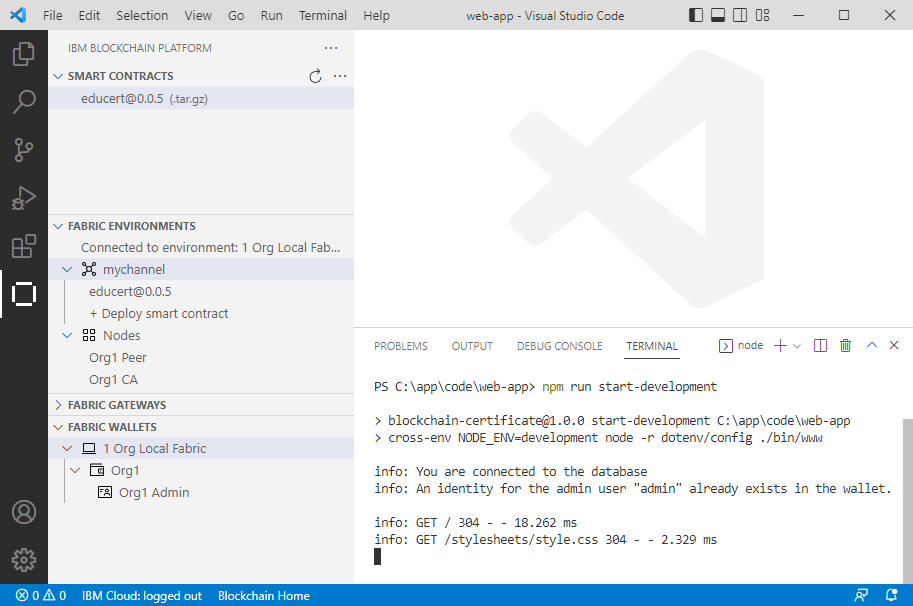
\includegraphics[width=.9\linewidth]{img/ide_start.PNG}
\caption{Chương trình Visual Studio Code}
\label{fig:ide_start}
\end{figure}

\section{Ứng dụng Web}


Giao diện ứng dụng web hoạt động tại địa chỉ http://localhost:3000/ như hình \ref{fig:main_vbcc}. 

\begin{figure}[H]
\centering
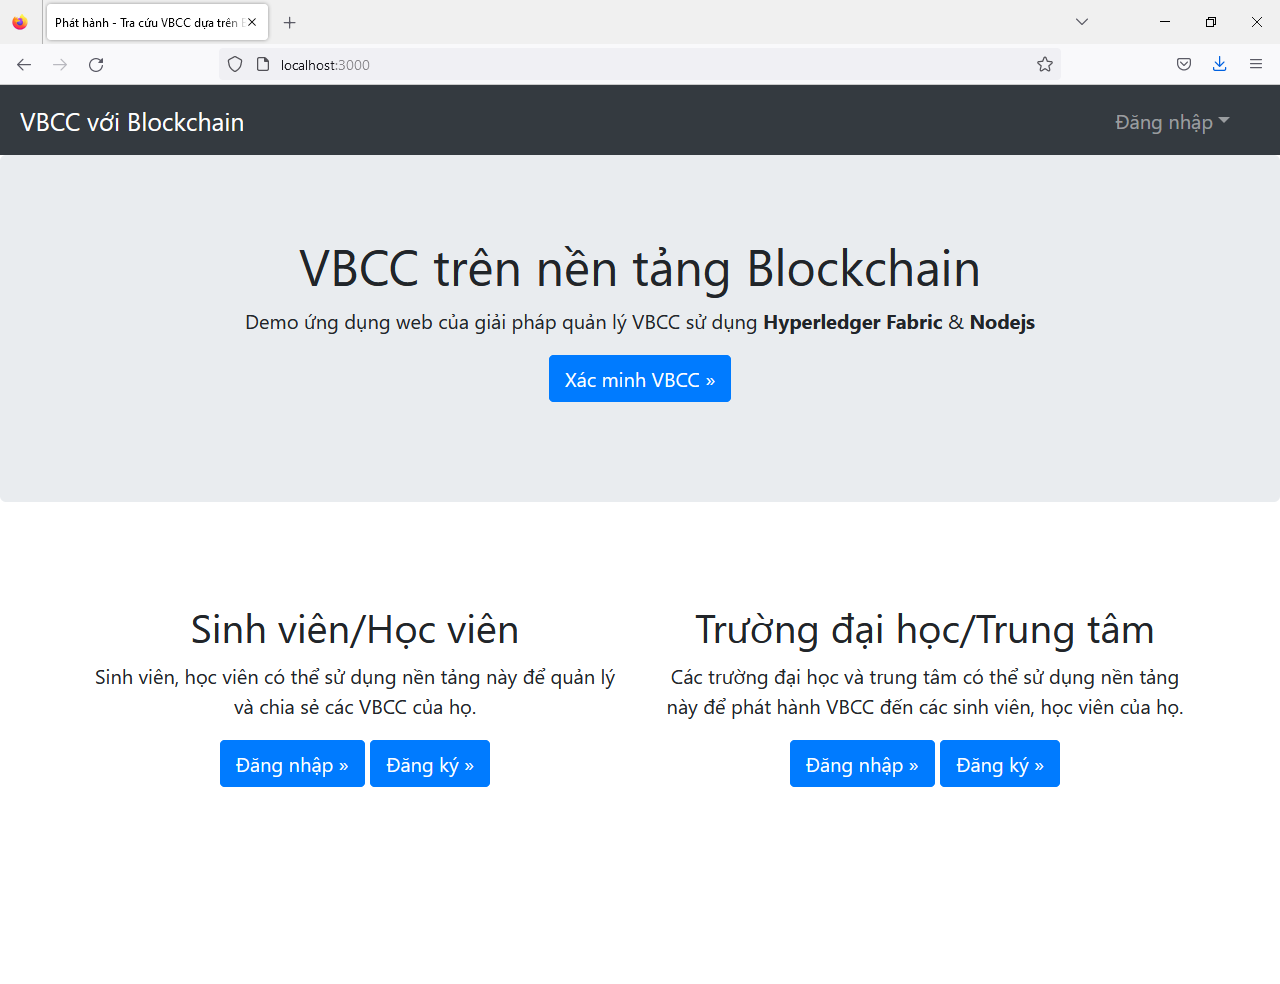
\includegraphics[width=.9\linewidth]{img/main_vbcc.png}
\caption{Giao diện hệ thống}
\label{fig:main_vbcc}
\end{figure}

\textbf{Màn hình chức năng quản lý VBCC của Trường, trung tâm}

\emph{Màn hình phát VBCC cho sinh viên}, hình \ref{fig:tt_phathanh}

Trường thực hiện đăng nhập sử dụng hệ thống. Sau đó, chọn chức năng phát VBCC. 

Sau đó nhập tất cả thông tin VBCC cần thiết để cấp VBCC, trong đó Email của Sinh viên được dùng để tạo mật mã VBCC.
\begin{figure}[H]
\centering
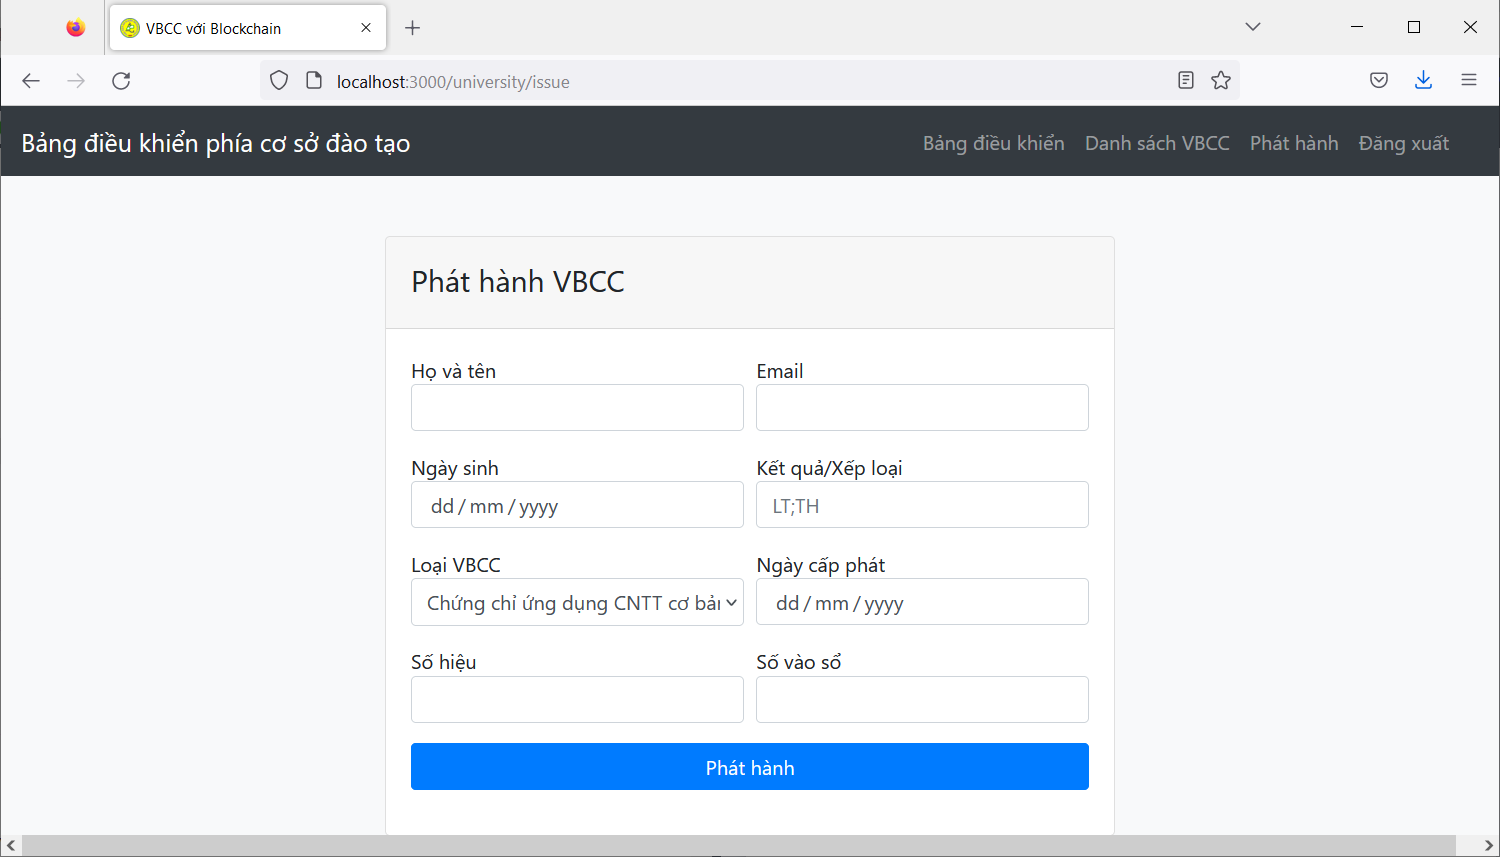
\includegraphics[width=.9\linewidth]{img/tt_phathanh.PNG}
\caption{Màn hình cấp VBCC cho sinh viên}
\label{fig:tt_phathanh}
\end{figure}

\emph{Màn hình xem các VBCC đã cấp cho sinh viên}  yêu cầu Trường thực hiện đăng nhập sử dụng hệ thống. Sau đó,  chọn chức năng xem VBCC. 

\begin{figure}[H]
\centering
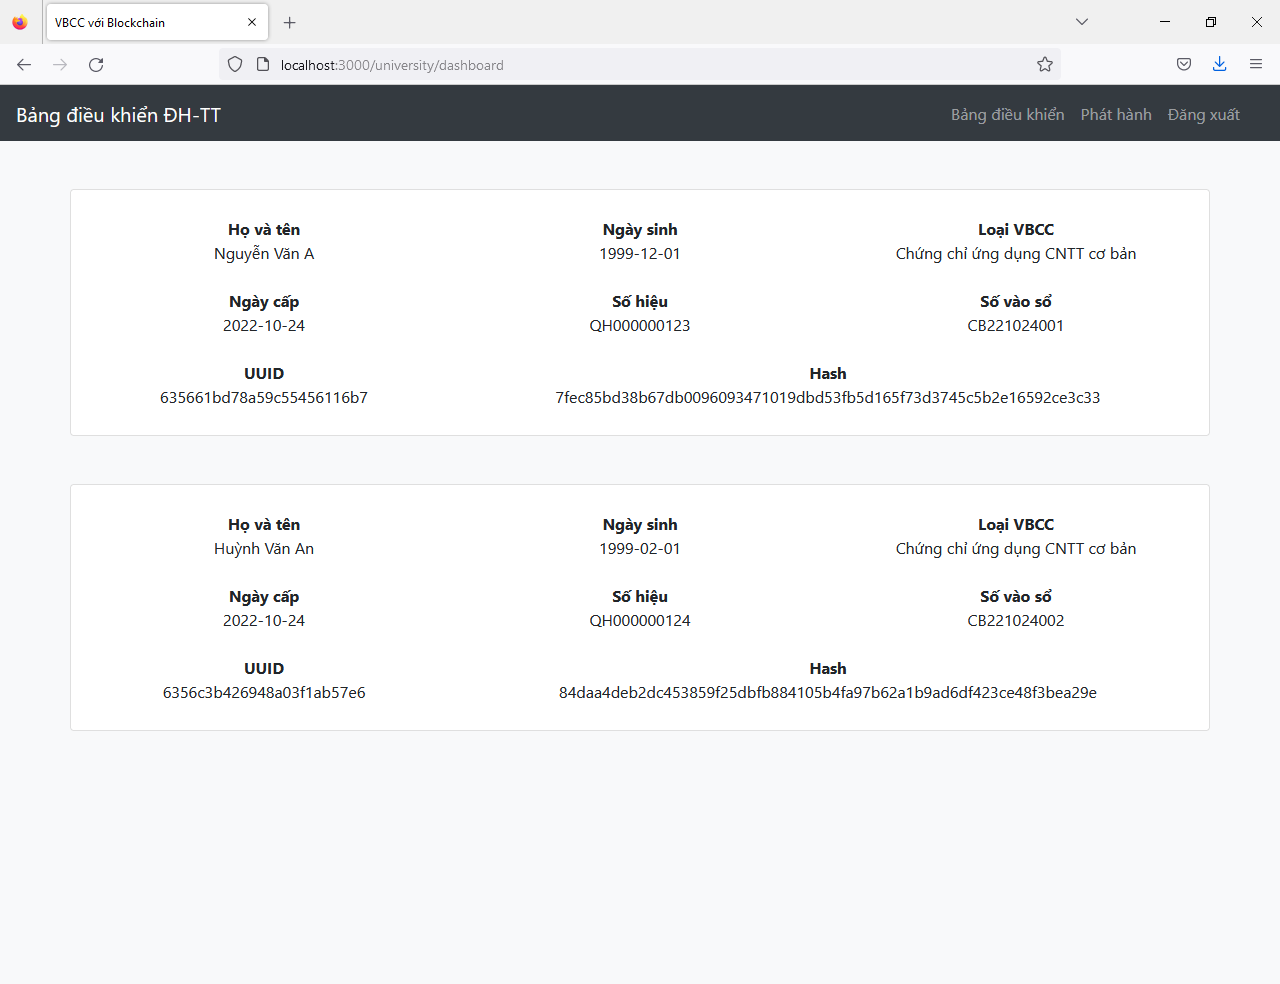
\includegraphics[width=.9\linewidth]{img/tt_dacap.PNG}
\caption{Màn hình xem các VBCC đã cấp}
\label{fig:tt_dacap}
\end{figure}


Sinh viên, học viên có chức năng

Màn hình đăng ký tài khoản.
Sinh viên cần đăng ký tải khoản để sử dụng hệ thống.
Sinh viên nhập thông tin đăng ký, trong đó Email sinh viên dùng để mật mã VBCC.

\begin{figure}[H]
\centering
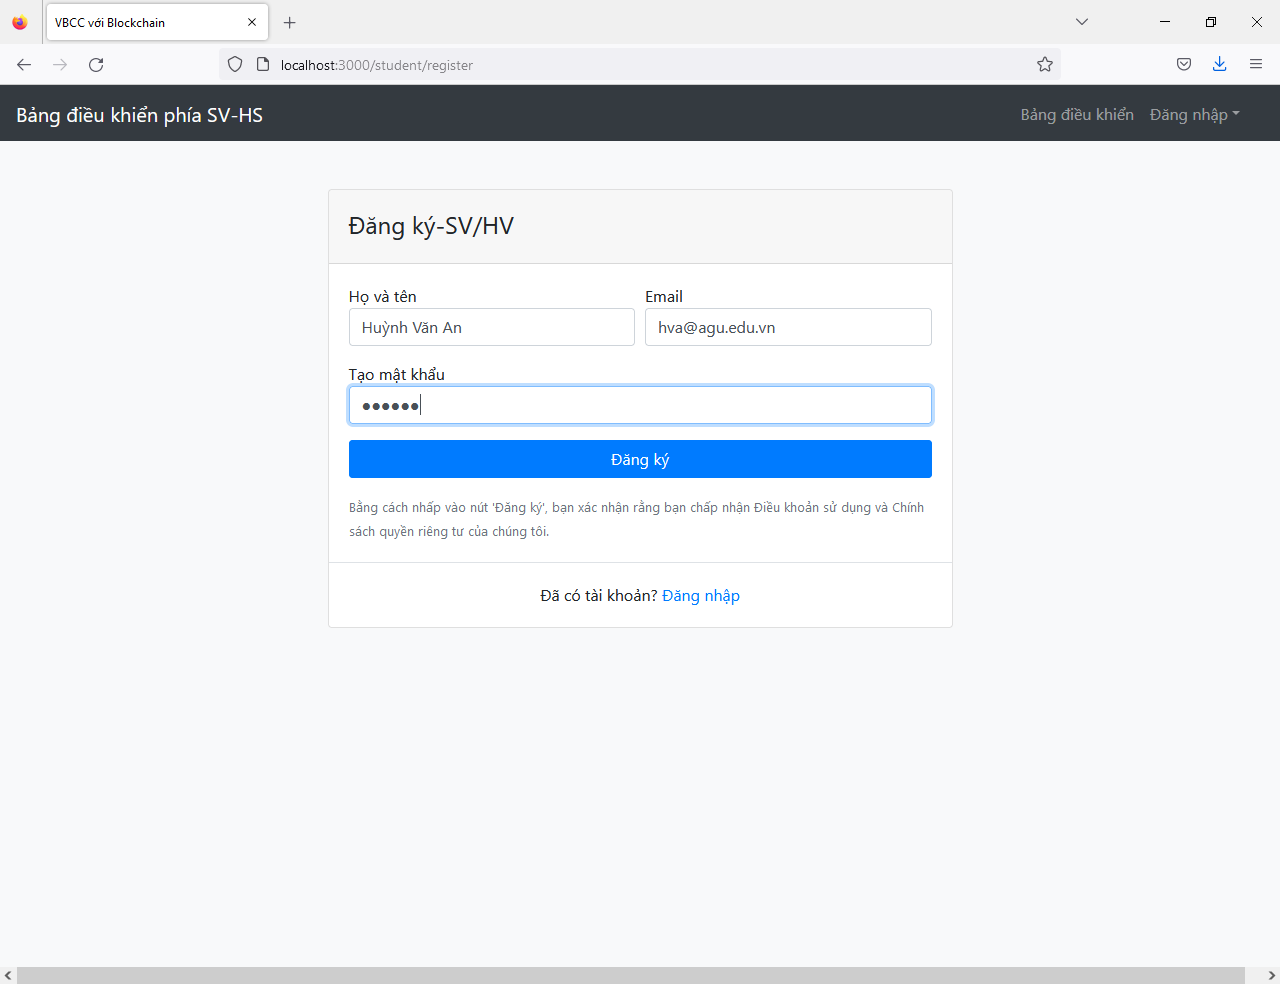
\includegraphics[width=.9\linewidth]{img/std_new.PNG}
\caption{Màn hình đăng ký tài khoản}
\label{fig:std_new}
\end{figure}

Màn hình xem các VBCC đã nhận.
Sinh viên cần đăng nhập tải khoản để sử dụng hệ thống.
Sinh viên chọn xem VBCC.
\begin{figure}[H]
\centering
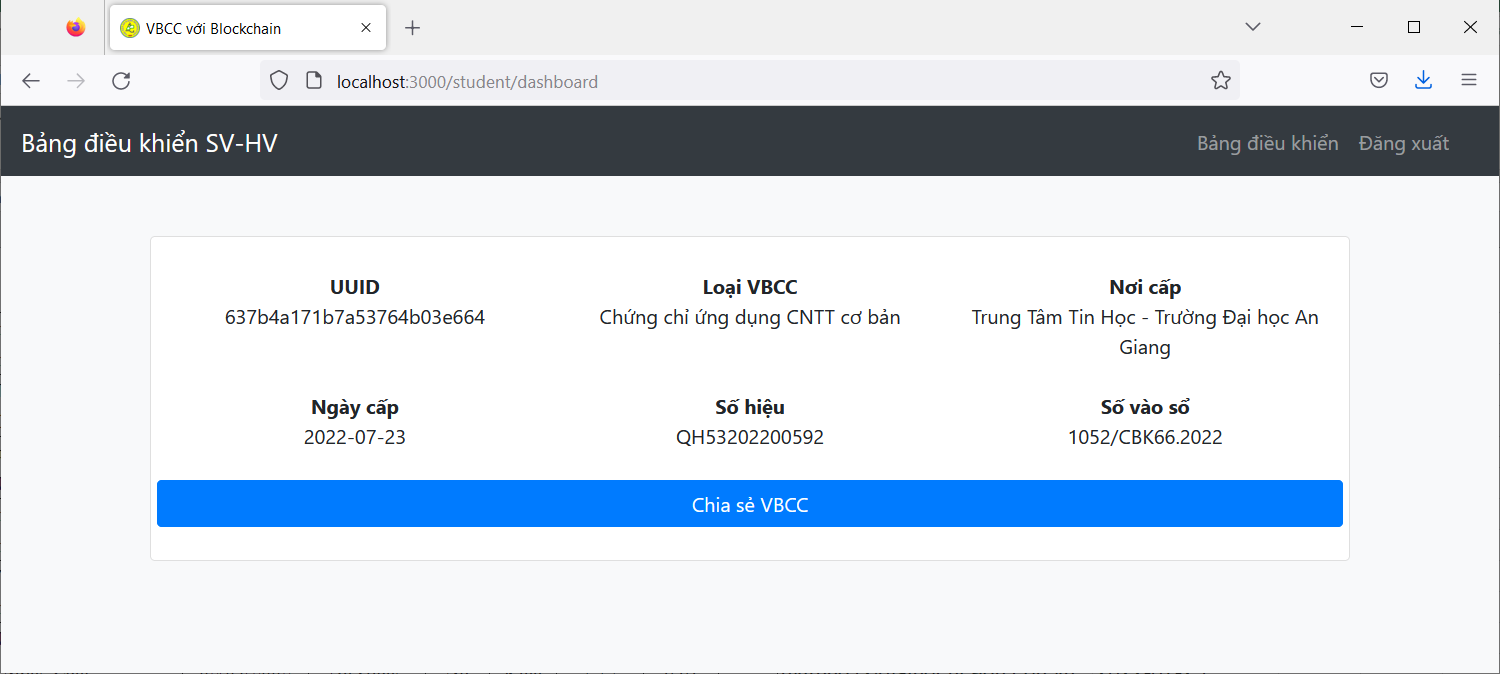
\includegraphics[width=.9\linewidth]{img/sv_hva.PNG}
\caption{Màn hình xem các VBCC đã nhận}
\label{fig:sv_hva}
\end{figure}

Màn hình chia sẻ VBCC đã nhận.
Sinh viên cần đăng nhập tải khoản để sử dụng hệ thống.
Sinh viên chọn chức năng chia sẻ VBCC.
\begin{figure}[H]
\centering
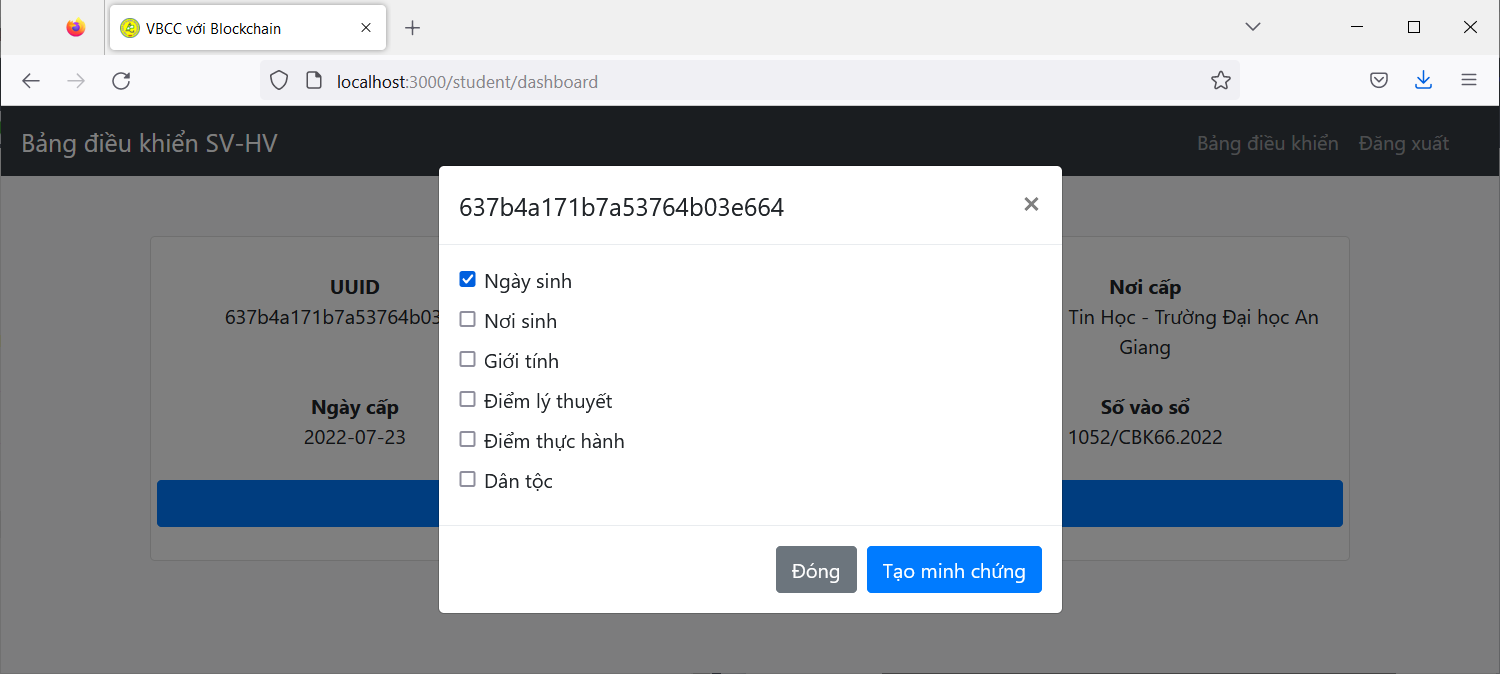
\includegraphics[width=.9\linewidth]{img/sv_chiase.PNG}
\caption{Màn hình chia sẻ thông tin VBCC}
\label{fig:sv_chiase}
\end{figure}

Màn hình chọn thông tin cá nhân chia sẻ.
Sinh viên cần đăng nhập tải khoản để sử dụng hệ thống.
Sinh viên chọn chức năng chia sẻ VBCC.
Sinh viên chọn những thông tin cá nhân cần chia sẻ.
\begin{figure}[H]
\centering
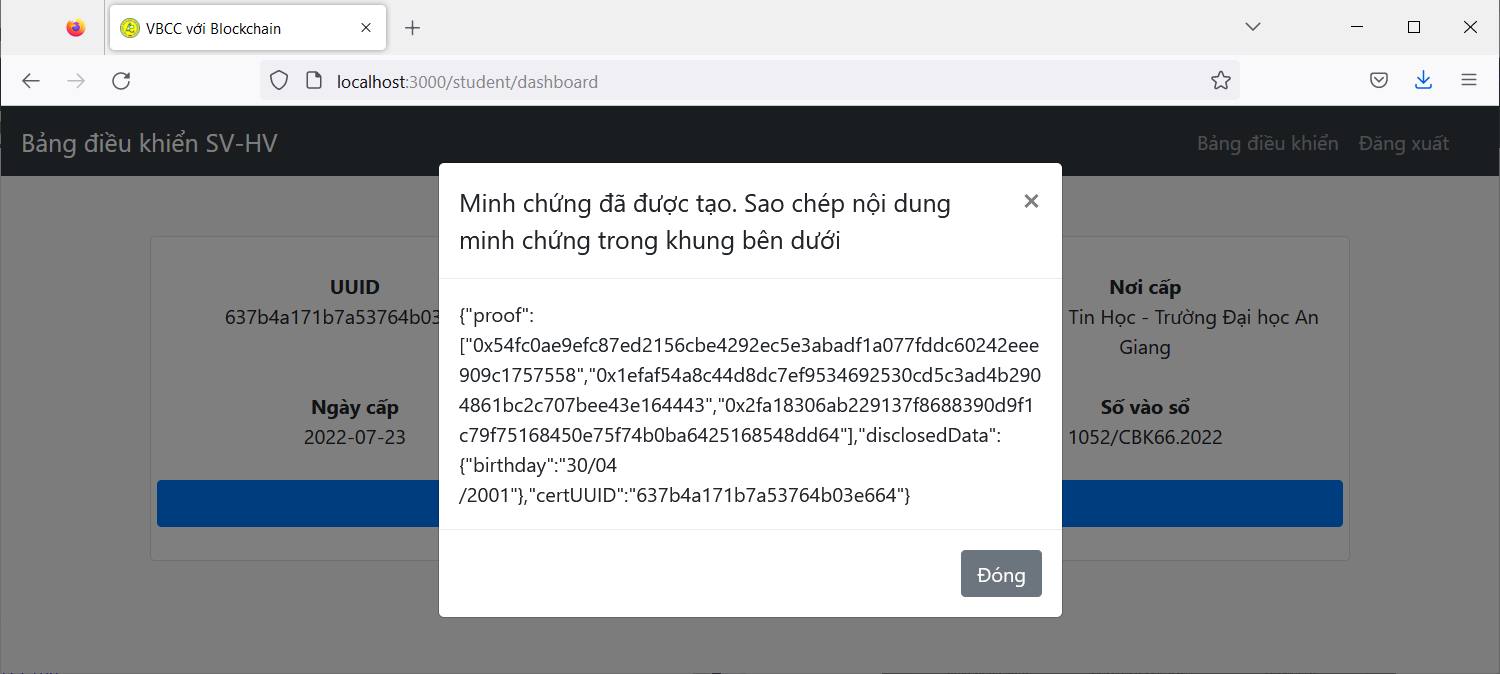
\includegraphics[width=.9\linewidth]{img/sv_minhchung.PNG}
\caption{Màn hình hiển thị mã xác thực VBCC}
\label{fig:sv_minhchung}
\end{figure}

Đơn vị xác minh chứng chỉ có chức năng

\begin{figure}[H]
\centering
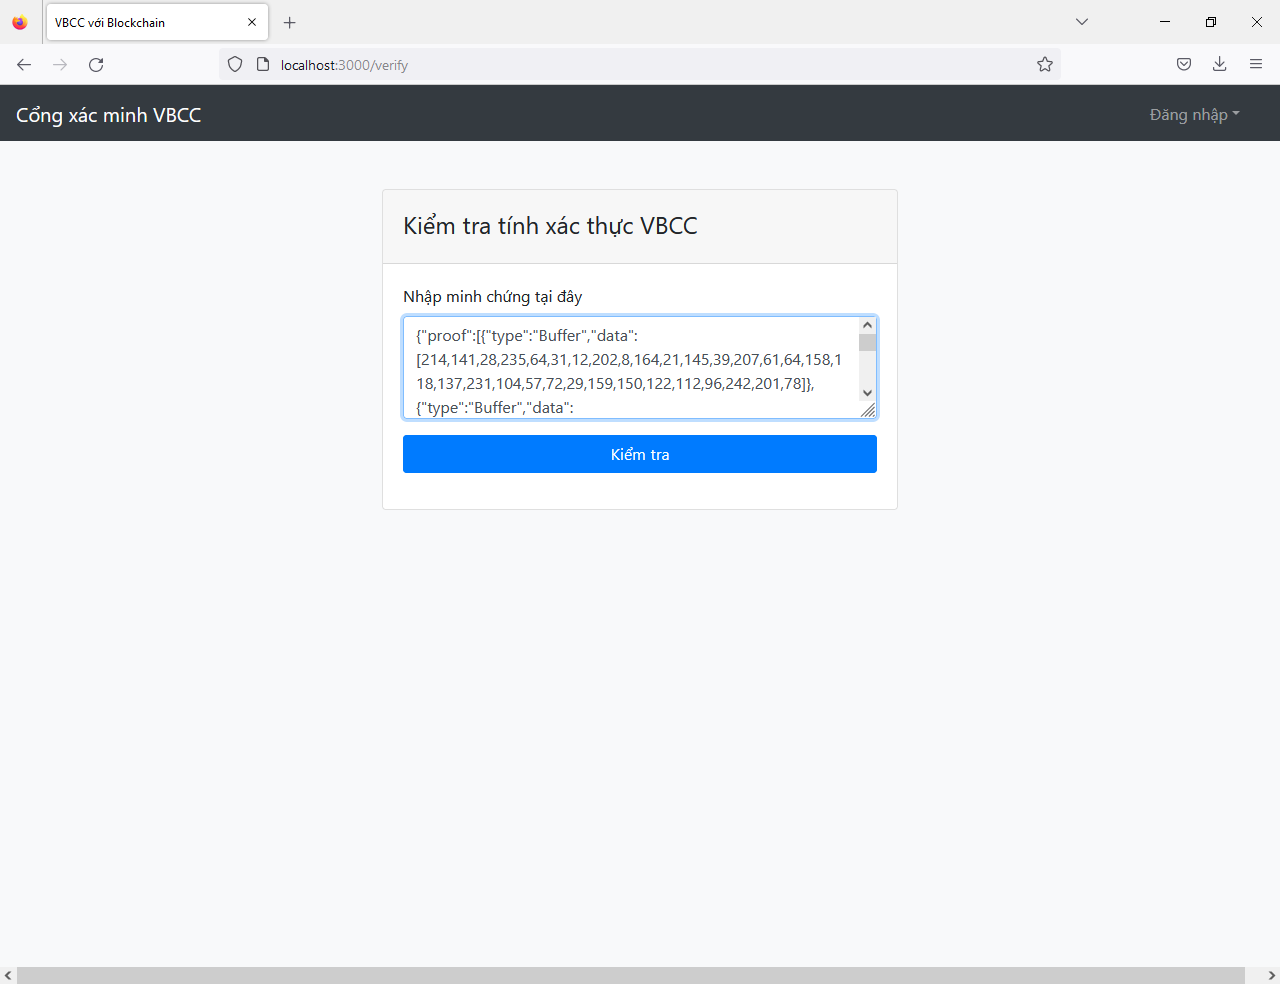
\includegraphics[width=.9\linewidth]{img/v_begin.PNG}
\caption{Màn hình nhập mã xác thực VBCC}
\label{fig:v_begin}
\end{figure}


